\chapter{Hybrid Solver}\label{chapter:hybrid_solver}

In this work, we use \acrshortpl{acr:GPU} to accelerate spectral methods. We use
\acrshortpl{acr:GPU} because they have a higher parallel throughput that traditional
\acrshortpl{acr:CPU}. We have shown that we can gain up to around three times the performance of
\acrshortpl{acr:CPU} on \acrshort{acr:HPC} systems in Section~\ref{section:results:scaling_tests}.

By that metric, by using only \acrshortpl{acr:GPU} we leave \(25 \% \) of the performance of those
systems on the table. While we perform computations on \acrshortpl{acr:GPU}, each \acrshort{acr:GPU}
is paired with a \acrshort{acr:CPU} core to feed it data and instructions, while the other
\acrshort{acr:CPU} cores are left idle. If we could design a program that uses both
\acrshortpl{acr:GPU} and \acrshortpl{acr:CPU} for computations, we could unlock the full processing
power of those \acrshort{acr:HPC} systems. This appendix describes a heterogeneous \textit{hybrid
solver} that uses both \acrshortpl{acr:CPU} and \acrshortpl{acr:GPU} to compute the solution.

In this work, we implemented a \acrshort{acr:CPU} version of the program to perform the
\acrshort{acr:CPU}-\acrshort{acr:GPU} comparison for Section~\ref{section:results:scaling_tests}.
Both versions use the same interface to communicate between processes via \acrshort{acr:MPI}, which
means it was simple to make them work together heterogeneously. To pick the kind of worker a process
is, we launch multiple processes via \acrshort{acr:MPI}. The first processes pick \acrshort{acr:GPU}
devices until there are none remaining in the system and execute the \acrshort{acr:GPU} version of
the code, and the remaining processes execute the \acrshort{acr:CPU} version of the code.

The work now needs to be partitioned between \acrshortpl{acr:CPU} and \acrshortpl{acr:GPU}. Since
those two types of processors have vastly different capabilities, the partition must be uneven in
order to obtain the best performance. Section~\ref{section:load_balancing:workload_leveling}
describes the algorithm to repartition a 1D workload. At the end of the section, we make the
assumption that all workers have the same capacity to simplify the equation. This is no longer the
case if we can have both \acrshort{acr:CPU} and \acrshort{acr:GPU} workers. We will use
Equation~\ref{equ:ideal_workload} to separate the work between workers. It states:

\begin{equation}
	w_{ideal,p} = W \frac{c_p}{C},
\end{equation}

\noindent
where \(W\) is the total workload, \(C\) is the total capacity, \(p\) is a worker index, \(c_p\) is
the capacity of worker \(p\), and \(w_{ideal,p}\) is the ideal workload for worker \(p\). We can
easily find \(W\) by summing the number of elements in the problem, and \(C\) by summing the
capacity of each worker. The capacity of each worker, representing the relative speed at which it
solves problems or the number of elements it can compute in the same time as others, is the only
unknown. This is the quantity that must be different for \acrshortpl{acr:CPU} and
\acrshortpl{acr:GPU}.

For the purpose of this quick exploration of hybrid solvers, we will use a simple heuristic to
determine the relative capacity of \acrshortpl{acr:CPU} and \acrshortpl{acr:GPU}. We run a simple
case with one \acrshort{acr:GPU} and time its execution, then do the same with a single
\acrshort{acr:CPU}. This gives us the performance ratio between the two types of workers. On the
consumer platform described in Subsection~\ref{subsection:results:platforms:consumer}, the ratio
amounts to about \(16\). This means that a \acrshort{acr:GPU} solves the problem \(16 \times \)
faster that a single \acrshort{acr:CPU} core, and should solve it in the same time as \(16\)
\acrshort{acr:CPU} cores. We give a capacity of \(16\) to \acrshort{acr:GPU} workers, and of one to
\acrshort{acr:CPU} workers.

We use the same test case from Section~\ref{section:results:test_case} to examine the hybrid version
of the program. We use the platform described in
Subsection~\ref{subsection:results:platforms:consumer}, with \(32\) \acrshort{acr:CPU} cores and one
\acrshort{acr:GPU}. We use a mesh with \(64\) elements in the \(x\) and \(y\) direction, and a
polynomial order \(N\) of four. Figure~\ref{fig:hybrid_load_balancing} shows the mesh partitioning
after load balancing.

\begin{figure}[H]
	\centering
	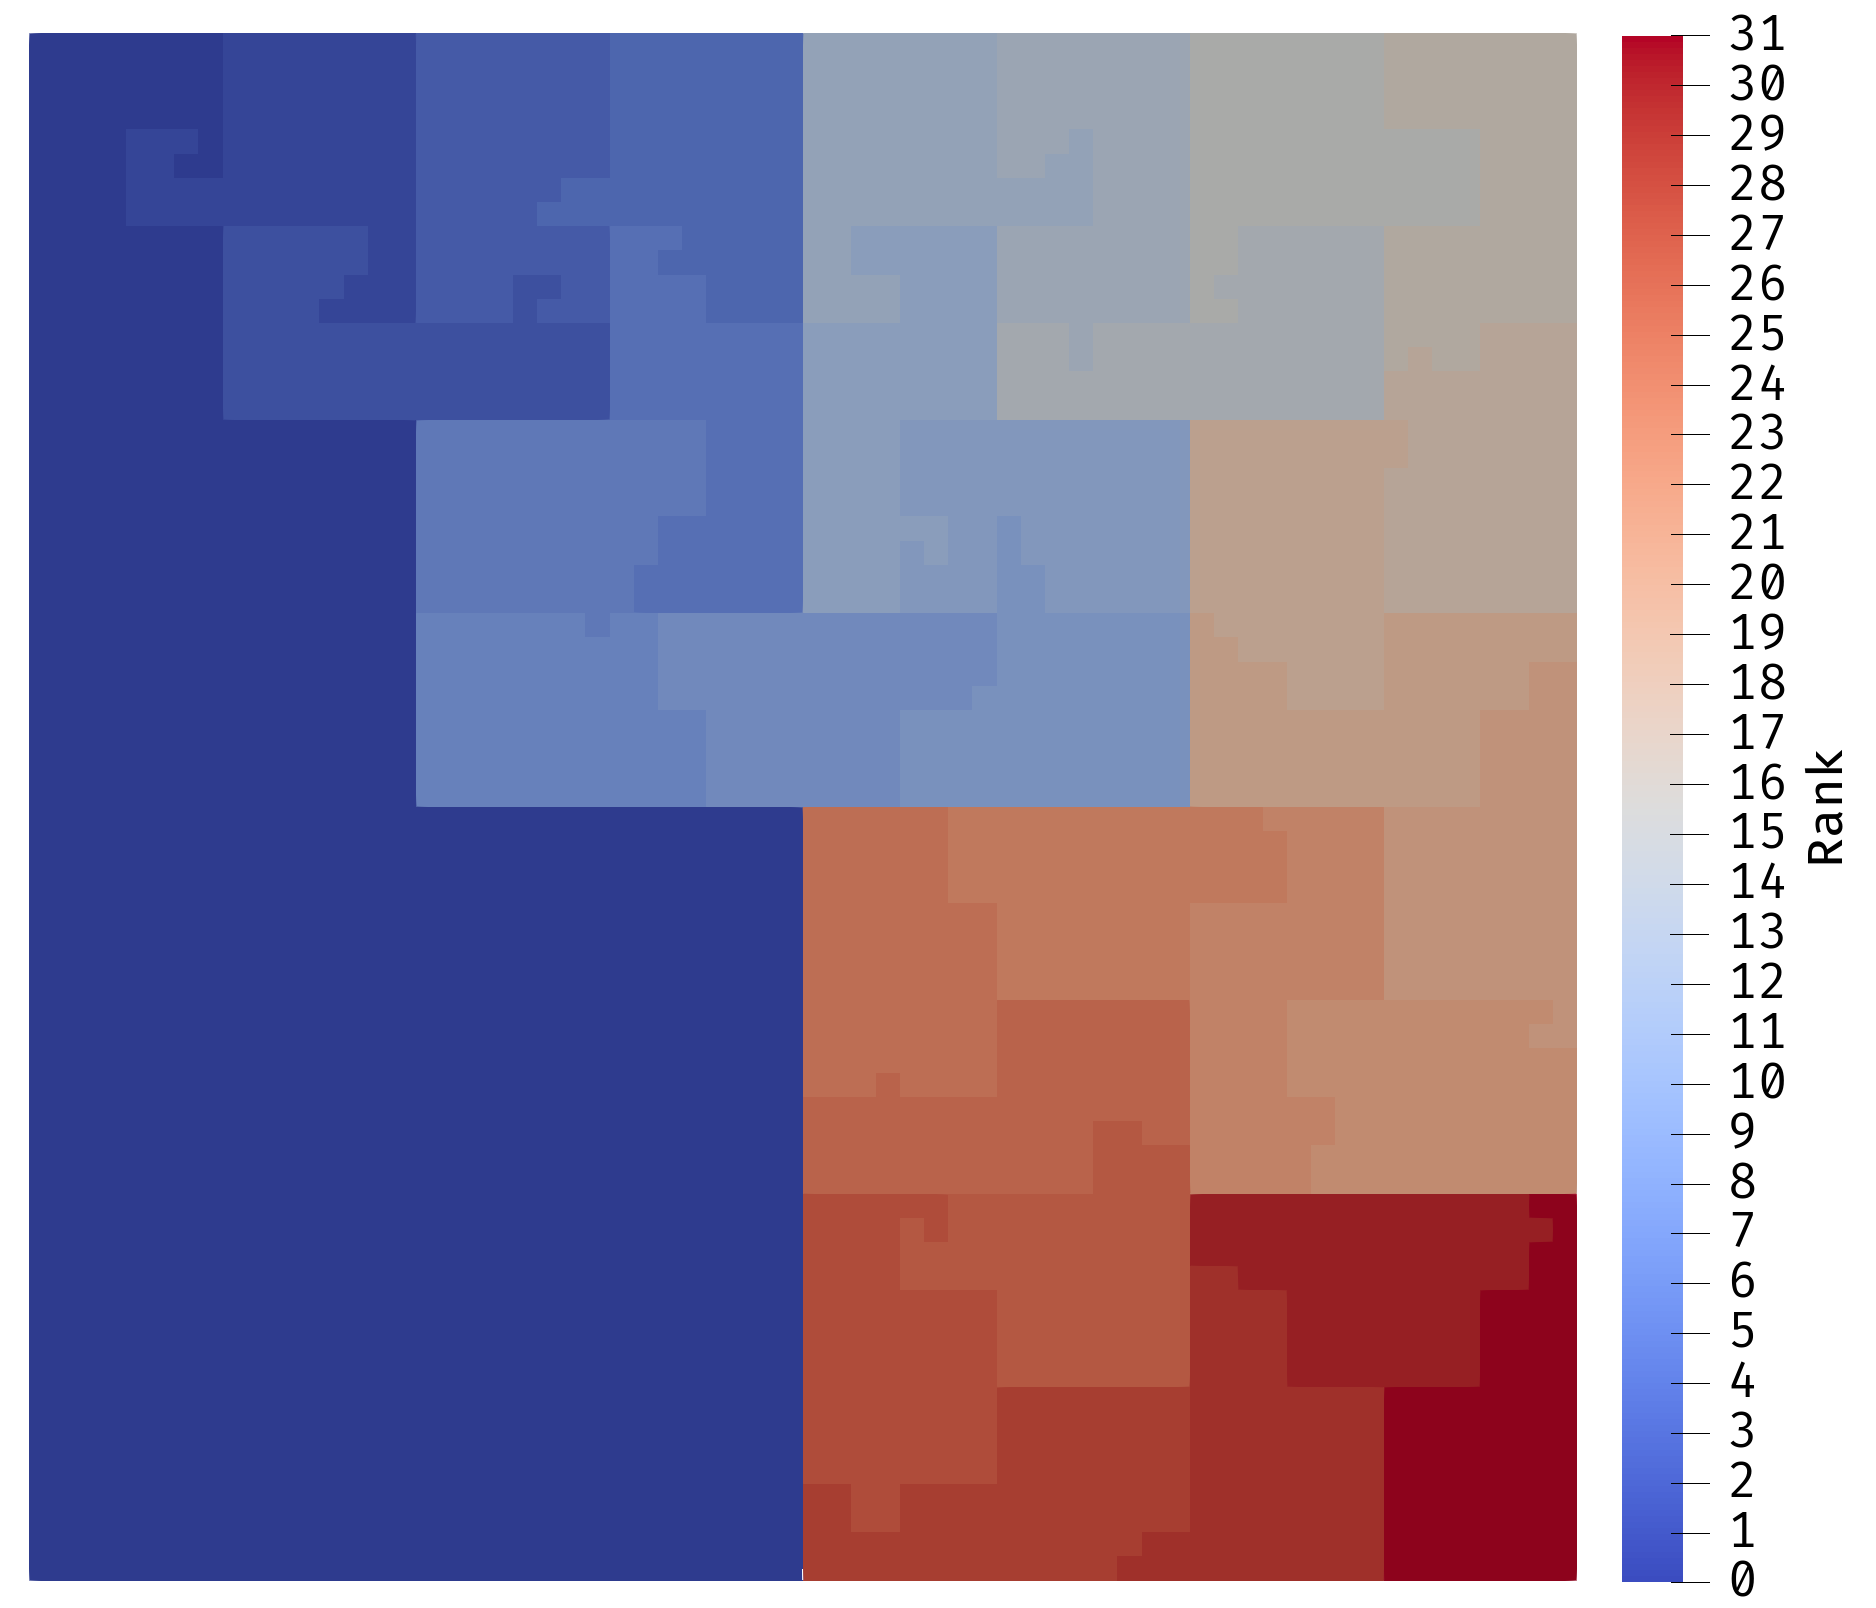
\includegraphics[width=0.65\textwidth]{Chapter_hybrid_solver/media/cpu_gpu}
	\caption{Load balancing with heterogenous workers: The first worker is a \acrshort{acr:GPU} and has more elements in its mesh block.}\label{fig:hybrid_load_balancing}
\end{figure}

Figure~\ref{fig:hybrid_load_balancing} shows that the first worker, with a rank of zero, has much
more elements in its mesh block than the other workers. The first worker is a \acrshort{acr:GPU},
and as such should have \(16\) times as many elements as the other workers. Along with \(31\)
\acrshort{acr:CPU} workers with a weight of one each, the \acrshort{acr:GPU} worker should have
about one third of the total elements of the mesh. The partitioning seen on the figure corroborates
this. 

In this case, the time for the hybrid solver was only faster than the \acrshort{acr:CPU} and
\acrshort{acr:GPU} solvers when computed with a relative capacity of \(4\) instead of \(16\). This
is possibly linked to the fact that the \acrshort{acr:GPU} is no longer optimally loaded since it
only has part of the elements compared to the comparison case used to determine the capacity. More
work will need to be performed in order to find the optimal capacities. The fact that the platform
used for testing only has a consumer-level \acrshort{acr:GPU} is probably also influencing the
results. 

Two limitations should be addressed before this hybrid solver becomes a real solution: the meshes
are initially partitioned equally, and we have to use heuristics for the capacity of different
workers. 

Currently, the program is made to accept as an input already-partitioned meshes when executed on
multiple workers. The majority of those multi-block meshes will be partitioned such that each block
has the same complexity. A mesh partitioner is provided with the program, and splits single-block
meshes into multi-block meshes, with each block having the same numbers of elements. This poses no
problem with a \acrshort{acr:GPU}-only or \acrshort{acr:CPU}-only solver, as all the workers will be
the same. With a hybrid solver, this means that the mesh will be far from ideal until load balancing
is performed, as the \acrshort{acr:GPU} and \acrshort{acr:CPU} will have the same number of
elements. One solution is to perform load-balancing once before starting the problem, but this
increases the computation time each time the program is launched. A second solution is to partition
meshes with the worker topology in mind, and produce already load-balanced meshes. This does not
work for meshes that are already in multi-block format, and makes the meshes specific to a
particular topology. The meshes would have to be re-partitioned for each worker topology, or simply
partitioned as part of the main program on each launch. As the overhead of load-balancing is low,
the first option is probably the best.

The second issue is that we have to run cases in order to determine the relative capacities of
\acrshortpl{acr:CPU} and \acrshortpl{acr:GPU}. The relative capacities depend on the specific
\acrshort{acr:GPU} and \acrshort{acr:CPU} models, and should be computed again for each computer
platform. More than that, it depends on the problem as the amount of mesh refinement and
polynomial order changes the performance ratio between \acrshortpl{acr:CPU} and
\acrshortpl{acr:GPU}. To get the best performance, we therefore would need to run each case on
\acrshortpl{acr:CPU}, then on \acrshortpl{acr:GPU} before we can compute it on both with the
computed capacities. This is tedious, and running each case three times completely negates any
performance gain brought by using a hybrid solver. The solution is to either use a ballpark value
for the relative capacities and have it be non-ideal in some cases, or compute it as the problem is
solved. This would imply timing each worker, and using the ratio between the time it took to compute
a number of iterations and the number of elements in its block  as its capacity. This way, the
capacity of each worker would be specific to its hardware and the current problem. It could even
change as the solution progresses, and be tailored to individual \acrshort{acr:CPU} cores or
\acrshortpl{acr:GPU} if there is a performance from unit to unit. It would also enable the program
to run on different types of computers at the same time, and make the program more robust.

All in all, a hybrid solver is a straightforward upgrade to make to increase the computational
resources available to solve problems. Some work remains to be done to make sure the work is
partitioned fairly between the heterogeneous workers, but even with approximated capacities the
hybrid solver shows promising results. This is definitely an interesting area of future work. 
